\section{Profiles Service}{Jose I. Retamal }

\indent
\indent
The profile service manages information about users, cities, and places. The data contained is editable by the users and provide information about them. 

The service is composed of the main service that connects to a Neo4j database using a Java DBA(Figure \ref{profiles:profilesmaindiagram}). The main service is design to be stateless; therefore, many instances of the service can be created for load balancing and scaling the system. 

There are relations between the different types of profiles that allow us to get data quickly and avoid the use of complicated queries.

\begin{figure}[H]
	\begin{center}
		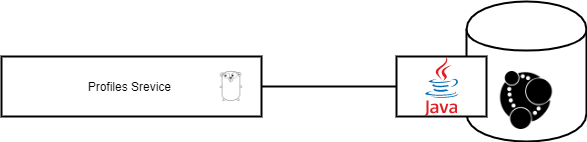
\includegraphics[width=120mm,scale=1]{img/profiles/profile-main-diagram.png}
		\caption{Profiles Service - Main UML.}
		\label{profiles:profilesmaindiagram}
	\end{center}
	
\end{figure}

\subsection{Request Sequence}

Each request contains a token that is checked with the authentication service if the token is valid, then the service access the database to serve the request(Figure \ref{profiles:reqeustsequence}).

\begin{figure}
	\begin{center}
		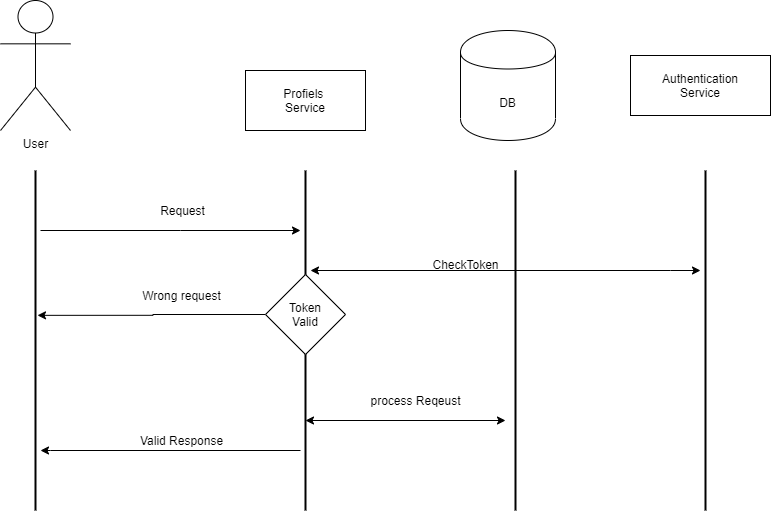
\includegraphics[width=120mm,scale=1]{img/profiles/profile-request-sequence.png}
		\caption{Profiles Service- Request Sequence.}
		\label{profiles:reqeustsequence}
	\end{center}
\end{figure}

\subsection{Endpoints}

\paragraph{Users}

\begin{itemize}
	\item Create User. This method is only called by the authentication service because users create an account using that service. The authentication service then sends the user data to the profiles service.
	
	\item	Get User. Get all data about the user.
	
	\item	Update a User. Updated the user.
\end{itemize}


\paragraph{City's}


\indent
Users create the cities; the user who creates a city can then update the data. A city can only be created once.



\begin{itemize}
	\item Create Cty.  Create the city and a relation between the user who creates the city and the city
	\item Visit City. Create a relation between the city and the user
	Update City. 
	\item Get City
	\item Get all Cities
\end{itemize}

\paragraph{Places}


\indent
Users create places; places belong to a city.

\begin{itemize}
	\item Create Place. Create the place and a relation between the user who creates the place and the place. Also, create a relation between the place and the city that belong.
	\item Visit Place. Create a relation between the place and the user/
	Update Place.
   \item	Get Place.
	\item Get All Place
\end{itemize}

\subsection{The Database}

\indent
\indent
The database is composed of three types of nodes: User, City, and Place(Figure \ref{profiles:dbuml}). Each node has a unique integer id. Users are also identified by the email, which is the unique id al over the system. A city can also be identified by the name and the country, place by name, the city that belongs, and the country(Figure \ref{profiles:dbnodes}).


\subsubsection{Relations}

\begin{itemize}
	\item  Places are in a City.  A relation between the city and the place, this relations allows us to retrieve quickly the places that belong to a city.
	
	\item Users visit cities and places. Create a relation between the user and the city/place. As users can mark several cities/places as visited, having this as a relation simplified the queries and give quick access to all cities/places that the user has visited.
\end{itemize}


\begin{figure}
	\begin{center}
		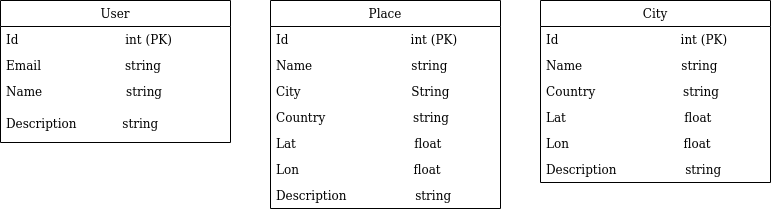
\includegraphics[width=120mm,scale=1]{img/profiles/profile-uml.png}
		\caption{Profiles Service- Neo4j DB Classes.}
		\label{profiles:dbuml}
	\end{center}
\end{figure}

\begin{figure}
	\begin{center}
		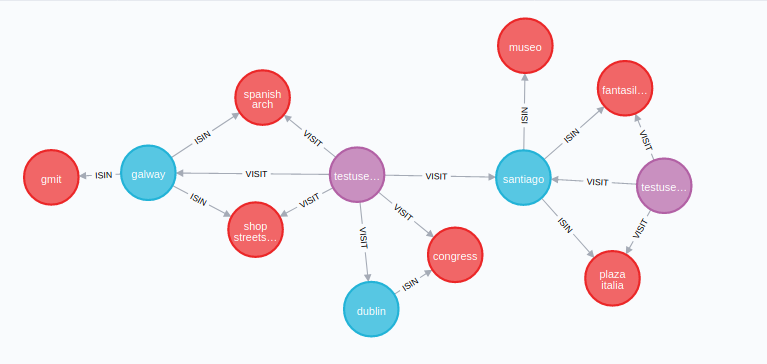
\includegraphics[width=120mm,scale=1]{img/profiles/neo4j-nodes.png}
		\caption{Profiles Service- Neo4j DB Dodes.}
		\label{profiles:dbnodes}
	\end{center}
\end{figure}
